\documentclass[russian,utf8,nocolumnxxxi,nocolumnxxxii]{eskdtext}
\usepackage[T1,T2A]{fontenc}
\usepackage[utf8]{inputenc}
\usepackage{amssymb,amsmath}
\usepackage{tikz}
\usepackage{siunitx}
\usepackage[american,cuteinductors,smartlabels]{circuitikz}
\usepackage[backend=biber]{biblatex}
\addbibresource{error_estimation_otchet.bib}
\usepackage[]{hyperref}
\hypersetup{colorlinks=true,}
\usepackage{textcomp}
\usepackage{booktabs}
\newcommand{\No}{\textnumero}
\ESKDdepartment{Федеральное агенство по побразованю}
\ESKDcompany{СПбГЭТУ}
\ESKDtitle{Пояснтельня записка к курсовой работе}
\ESKDsignature{Вариант N 32}
\ESKDauthor{Веренёв А.А.}
\ESKDchecker{Прокшин А.Н.}
\ESKDdocName{по дисциплине "Информатика"}
\begin{document}
\begin{center}
МИНОБРНАУКИ РОССИИ
\\САНКТ-ПЕТЕРБУРГСКИЙ ГОСУДАРСТВЕННЫЙ
\\ЭЛЕКТРОТЕХНИЧЕСКИЙ УНИВЕРСИТЕТ
\\«ЛЭТИ» ИМ. В.И. УЛЬЯНОВА (ЛЕНИНА)
\\Кафедра робототехники и автоматизации производственных систем
\vspace{30ex}
\\Пояснительная записка
\\к курсовой работе
\\по дисциплине «Информатика»
\vspace{40ex}
\\Санкт-Петербург
\\2018
\end{center}




\begin{document}
{\bfСодержание}
\\1. Цель и тема курсовой работы
\\2. Задание на курсовую работу
\\3. Введение
\\4. Исследование функции
\\5. Исследование кубического сплайна
\\6. Задача оптимального распределения неоднородных ресурсов
\\7. Список литературы

\newpage
\section{Цель и тема курсовой работы}
 Уметь применять персональный компьютер и математические пакеты прикладных программ в инженерной деятельности.
\\{\bfТема курсовой работы:} решение математических задач с использованием математического пакета «SciLab» и системы компьютерной алгебры «Reduce».

\newpage
\section{Введение}
В настоящее время при решении различных как прикладных инженерных, так и чисто исследовательских задач, возникает необходимость в использовании широкого круга алгоритмов из множества разделов математики. Между тем самостоятельная реализация многих алгоритмов на некотором языке программирования может быть сложна и избыточна. Вследствие этого широкое распространение получили математические пакеты и системы компьютерной алгебры, такие как: MatLab, Octave, SciLab, Mathematica, Reduce, Mapple, призванные избавить пользователя от рутинных процедур, предоставить удобный интерфейс взаимодействия с уже написанным программным кодом и быстрым созданием нового. К сожалению, некоторые из перечисленных выше математических пакетов, будучи коммерческими по природе, имеют пакетом SciLab и системой компьютерной алгебры Reduce.

\newpage
\section{Задания на курсовую работу}
\\1. Даны функции $f(x)=\sqrt{3}sin(x)+cos(x),g(x)=cos(2x+\frac{\pi}{3})-1$
\\а)Решить уравнение f(x)=g(x).
\\б)Исследовать функцию h(x)=f(x)-g(x) на промежутке $[0;\frac{5\pi}{6}]$
\\2. Найти коэффициенты кубического сплайна, интерполирующего данные, представленные в векторах:\\
$V_{x}=[0,0.5,1.4,2.25,3.5]$
$V_{y}=[3.0,2.7,3.7,3.333,3.667]$\\
Построить на графике функции f(x),полученную после нахождения коэффициентов кубического сплайна. \\
Представить графическое изображение результатов интерполяции исходных данных различными методами с использованием встроенных функций
\\splin(x,y,“natural”), splin(x,y,“clamped”), splin(x,y,“not\_a\_knot”), splin(x,y, “fast”), splin(x,y,“monotone”), interp(xx,x,y,d)\\
3. Решить задачу оптимального распределения неоднородных ресурсов.
Требуется решить следующую задачу оптимального распределения неоднородных ресурсов. Пусть в распоряжении завода железобетонных изделий (ЖБИ) имеется m видов сырья (песок, щебень, цемент) в объемах ${\bf a_i}$ .Требуется произвести продукцию {\bf n} видов. Дана технологическая норма $c_ij$ требления отдельного i-го вида сырь для изготовления единицы продукции каждого j-го вида. Известна прибыль $\pi_j$ получаема от выпуска единицы продукции j-го вида. Требуется определить, какую продукцию и в каком количестве должен производить завод ЖБИ, чтобы получить максимальную прибыль.
\begin{table}[h!]
\centering
\begin{tabular}{l|l|l|l|l|l} 
\toprule
Используемые &\multicolumn{4}{c|}{Изготавливаемые изделия }& Наличие       \\ 
\cline{2-5}
ресурсы, a_i   & \:  И1  \:                 & \:   И2  \:                 &\: И3   \:                &\: И4 & ресурсов, a_i  \\ 
\hline
Трудовые      & \multicolumn{1}{c|}{4}                    & \multicolumn{1}{c|}{4}                    & \multicolumn{1}{c|}{4}                   & \multicolumn{1}{c|}{6}  & 14            \\
Материальные  & \multicolumn{1}{c|}{4}                   & \multicolumn{1}{c|}{6}                    & \multicolumn{1}{c|}{6}                    & \multicolumn{1}{c|}{3}  & 12            \\
Финансовые    & \multicolumn{1}{c|}{6}                    & \multicolumn{1}{c|}{4}                    & \multicolumn{1}{c|}{5}                    & \multicolumn{1}{c|}{8}  & 35            \\
Прибыль, П_j   & \multicolumn{1}{c|}{40}                   & \multicolumn{1}{c|}{55}                   & \multicolumn{1}{c|}{35}                   & \multicolumn{1}{c|}{25} &               \\
\bottomrule
\end{tabular}
\end{table}

\newpage
\section{Решение и исследование триганометрической функции}
Решение уравнение - поиск его корней\\
$h(x)=\sqrt{3}sin(x)+cos(x)-cos(2x+\frac{\pi}{3})+1$\\
Для нахождения корней есть два пути - численный и аналитический\\
{\bfЧисленное решение.}\\
Для нахождения численного решения воспользуемся функцией "fsolve".\\
Для начала построим график.\\
function y=h(x)\\
y=sqrt(3)*sin(x)+cos(x)-cos(2*x+\%pi/3)+1\\
endfunction\\
plot(0:0.01:2*\%pi,h)\\
Полученный график изображен на Рис.1.
\vspace{35mm}
\begin{center}
\begin{minipage}[h]{0.65\linewidth}
\center{\includegraphics[width=1\linewidth]{1.PNG}}  \\
\frametitle{ Рис 1. График функции h(x)}
\end{minipage}
\end{center}

\newpage
Изучив график, допустимо предположить наличие трех корней. Зададим приближные значения и воспользуемся функцией "fsolve".\\
\\x0 = [2.6,4.2,5.6];
\\$[x,v] = fsolve(x0,h)$

\vspace{35mm}
\begin{center}
\begin{minipage}[h]{0.65\linewidth}
\center{\includegraphics[width=1\linewidth]{3.PNG}}  \\
\frametitle{Корни функции h(x)}
\end{minipage}
\end{center}

\newpage
{\bfАналитическое решение.}\\
Для отыскания аналитического решения воспользуемся функцией solve из системы компьютерной алгебры «WolframAlpha»:\\
Упростим данное уравнение, воспользовавшись двумя тригонометрическими тождествами: $$sin(x+y)=sin(x)cos(y)+cos(x)sin(y)$$
$$cos(2x)=1-2sin^2(x) $$
$$\sqrt{3}sin(x)+cos(x),g(x)-cos(2x+\frac{\pi}{3})+1$$ $$=2(sin(x)cos(\frac{\pi}{6})+cos(x)sin(\frac{\pi}{6}))+2sin^2(x+\frac{\pi}{6})$$ $$=2(sin(x+\frac{\pi}{6})+sin^2(x+\frac{\pi}{6})$$\\
и получим тривиальное уравнение, эквивалентное исходному
$$2(sin(x+\frac{\pi}{6})+sin^2(x+\frac{\pi}{6})=0$$
Применим к нему функцию solve:\\
solve(2sin(x+pi/6)*(1+sin(x+pi/6)));
и получим решение:
\begin{center}
\begin{minipage}[h]{0.65\linewidth}
\center{\includegraphics[width=1\linewidth]{4.PNG}}  \\
\end{minipage}
\end{center}

\newpage
{\bfб)Исследовать функцию h(x)=f(x)-g(x) на промежутке $[0;\frac{5\pi}{6}]$ }\\
1)Иследование на четность или нечетность.
Если $f(-x)=f(x)$, то фунция четная. Если $f(-x)=-f(x)$ - нечетная. Если фунция не является четной или нечетной, то ее обычно называют - функцией общего вида.\\
\begin{center}
\begin{minipage}[h]{0.65\linewidth}
\center{\includegraphics[width=1\linewidth]{5.PNG}}  \\
\center{\includegraphics[width=1\linewidth]{6.PNG}}  \\
\center{\includegraphics[width=1\linewidth]{7.PNG}}  \\
\end{minipage}
\end{center}

\newpage
2) Построение графика иследуемой функции на промежутке $[0;\frac{5\pi}{6}]$ \\
\begin{center}
\begin{minipage}[h]{0.65\linewidth}
\center{\includegraphics[width=1\linewidth]{8.PNG}}  \\
\end{minipage}
\center{\includegraphics[width=1\linewidth]{9.PNG}}  \\
\end{center}

\newpage
3) Получение точек экстремума функции с помощью интерполяционной формулы Ньютона

Для выявления точки экстремума производная исследуемой функции должна быть равна нулю $h(x)=0$. При расчётах на исследуемый области $x=(0;\frac{5\pi}{6}$, ориентируясь по рисунку №2 видим что количество таких точек равно единице, поскольку поскольку функция в данном случае изгибается один раз.

\begin{figure}[h]
\center{\includegraphics[width=1\linewidth]{9.PNG}}
\caption*{График функции y=h(x)}
\label{ris:RS2.png}
\end{figure}



Поскольку точка экстремума являться h(x)=0, то в случае когда $h'(x)>0$ функция возрастает, а в случае $h'(x)<0$ функция убывает. Из расчётов было выявлено, что при х=1,048 функция $h'(x)<0$, следственно функция убывает после точки экстремума, на исследуемом промежутке. При х=1 функция $h'(x)>0$ больше нуля, следственно она возрастет.\\

\newpage
4) Точки перегиба\\
Для нахождения точек экстремума - необходимо взять врую производную от данной функции.\\
$h''(x)=-\sqrt3*sin(x)-cos(x)+4*cos(2*x + \frac{\pi}{3})$
Из графика функции следует что на исследуемом промежутке x = (0; 5π), имеются
две точи перегиба. Первая точка перегиба в районе значений x = (0; 0, 2), вторая
в районе значений x = (2; 2.2)\\


    
Основываясь на полученных результатах можно сказать, что функция:

1) Возрастает на (0,$\frac{\pi}{3}$)

2) Убывает на ($\frac{\pi}{3},5\frac{\pi}{6}$)

3) Область определения функции $h(x) \in R$. 

4) Вертикальные и горизонтальные асимптоты отсутствуют.

5) функция является общей направленности.

6) Имеет глобальный максимум в точке $x=0$

7) Имеет глобальный минимум в точке $x=5\frac{\pi}{6}$

8) Точки перегиба x=0.111 и x=1.193

\newpage
\section{Исследование кубического сплайна}
\subsubsection{Задания и исходные данные для решения}
      $ $1. Найти коэффициенты кубического сплайна, интерполирующего данные, представленные в векторах$\,\,  {\vec{V}_x} \,\,$и$\,\, {\vec{V}_y.}$ \\
      $ {\,\,\,\,\,\,\,\,\,\,\,\,\,\,\,\,\,\,}$2. Построить на одном графике: функцию$\,\, {f(x)}\,\, $и$\,\,  функцию {f_1(x)}, $полученную после нахождения коэффициентов кубического сплайна.$ $ \\
      $ {\,\,\,\,\,\,\,\,\,\,\,\,\,\,\,\,\,\,}$3. Представить графическое изображение результатов интерполяции исходных данных$ $.\\

      $\vec{V}_x=\left(\begin{array}{c}0\\0.5\\1.4\\2.25\\3.5\end{array}\right),
      \,\,\,\vec{V}_y=\left(\begin{array}{c}3\\2.7\\3.7\\3.333\\3.667\end{array}\right)$ \\\\
      $ {\,\,\,\,\,\,\,\,\,\,\,\,\,\,\,\,\,\,}$Необходимо оценить погрешность в точке $ {x = 2.4}. $\,\,\,\,\,Вычислить значение функции в точке $\,{x = 1.2}.$\\
\newpage
      \subsubsection{Теория и вывод уравнения сплайна}
      Уравнение сплайна находится по пяти точкам\\
      $(x_1;y_1), (x_2;y_2), (x_3;y_3), (x_4;y_4), (x_5;y_5)$\\
      Представим сплайн полиномом третьей степени на каждом отрезке
      $[x_i, x_{i+1}]$.

      \begin{equation}\label{eq:F_i(x)}
      F_i(x)=A_i0+{A_{i1}}x+{A_{i2}}x^2+{A_{i3}}x^3,
      \end{equation}

      $где $x$ \in {\,} $[{x_i},{x_{i+1}}].$\\[4pt]
      Найдем коэффициенты $A_{ij}$ исходя из того, что в точках склейки функция не имеет разрывов, изломов и изгиб ее слева и справа совпадает. \\
      На каждом из отрезков $[x_i, x_{i+1}]$ график $F_i(x)$ проходит через точки $y_i$, $y_{i+1}.$
      \begin{equation}\label{eq:y_i}
      y_i=A_{i0}+{A_{i1}}{x_i}+{A_{i2}}{x_i}^2+{A_{i3}}{x_i}^3
      \end{equation}

      Получаем $8$ уравнений:
      \begin{equation}\label{eq:y1(x)}
      \begin{aligned}
      y_1=A_{10}+{A_{11}}{x_1}+{A_{12}}{{x_1}^2}+{A_{13}}{x_1}^3\\[4pt]
      y_2=A_{10}+{A_{11}}{x_2}+{A_{12}}{x_2}^2+{A_{13}}{x_2}^3\\[4pt]
      y_2=A_{20}+{A_{21}}{x_2}+{A_{22}}{x_2}^2+{A_{23}}{x_2}^3\\[4pt]
      y_3=A_{20}+{A_{21}}{x_3}+{A_{22}}{x_3}^2+{A_{23}}{x_3}^3\\[4pt]
      y_3=A_{30}+{A_{31}}{x_3}+{A_{32}}{x_3}^2+{A_{33}}{x_3}^3\\[4pt]
      y_4=A_{30}+{A_{31}}{x_4}+{A_{32}}{x_4}^2+{A_{33}}{x_4}^3\\[4pt]
      y_4=A_{40}+{A_{41}}{x_4}+{A_{42}}{x_4}^2+{A_{43}}{x_4}^3\\[4pt]
      y_5=A_{40}+{A_{41}}{x_5}+{A_{42}}{x_5}^2+{A_{43}}{x_5}^3\\[4pt]
      \end{aligned}
      \end{equation}
       Производные первого порядка во внутренних точках ${x_i}$ должны совпадать,
       т.е. производная слева
       $${{F_i}^{'}}({x_i}) = A_{i1}+ 2{A_{i2}}{x_i}+ 3A_{i3}{{x_i}^2}$$
        должна быть равна производной справа
        $${{F^{'}}_{(i+1)}}({x_i}) = {A_{{(i+1)}1}}+ 2{A_{{(i+1)}2}}{x_i}+ 3A_{{(i+1)}3}{{x_i}^2}$$
      Физический смысл равенства производных состоит в том, что в точках склейки у нас нет излома сплайна.
    \begin{equation}\label{eq:y^{'}(x)}
    \begin{aligned}
    A_{11}+ 2A_{12}{x_2}+ 3A_{13}{{x_2}^2}=A_{21}+ 2A_{22}{x_2}+ 3A_{23}{{x_2}^2}\\
    A_{21}+ 2A_{22}{x_3}+ 3A_{23}{{x_3}^2}=A_{31}+ 2A_{32}{x_3}+ 3A_{33}{{x_3}^2}\\
    A_{31}+ 2A_{32}{x_4}+ 3A_{33}{{x_4}^2}=A_{41}+ 2A_{42}{x_4}+ 3A_{43}{{x_4}^2}\\
    \end{aligned}
    \end{equation}

      Производные второго порядка в точках склейки ${x_i}$ должны совпадать,
      т.е. вторая производная слева
      $${{F_i}^{''}}{(x_i)} = 2{A_{i2}}+ 6{A_{i3}}{x_i}$$
      должна быть равна второй производной справа
      $${{F^{''}}_{(i+1)}{(x_i)} =2{A_{{(i+1)}2}+ 6{A_{{(i+1)}3}}{x_i}$$
         Физический смысл равенства вторых производных состоит в том, что в точках склейки изгиб сплайна справа и слева должен быть одинаковым.

      		\begin{equation}\label{eq:y^{'}(x)}
      		\begin{aligned}
      		2{A_{12}}+ 6{A_{13}}{x_2}=2{A_{22}}+ 6{A_{23}}{x_2}\\
      		2{A_{22}}+ 6{A_{23}}{x_3}=2{A_{32}}+ 6{A_{33}}{x_3}\\
      		2{A_{32}}+ 6{A_{33}}{x_4}=2{A_{42}}+ 6{A_{43}}{x_4}\\
      		\end{aligned}
      		\end{equation}
      		
      		Еще два уравнения - из граничных условий в крайних точках $x_1$, $x_n$:
      	\begin{equation}\label{eq:F^{''}(x)=0}
      	\begin{aligned}
      	{C_{11}}{F^{'}}{x_1}+{C_{12}}+ {{F^{''}}{(x_1)}={C_{13}}\\
      	C_{n1}{F^{'}}{n_1}+C_{n2}+ {{F^{''}}{(n_2)}=C_{n3}\\
      	\end{aligned}
      	\end{equation}
      						
      Найдем график сплайна в случае, когда концы сплайна оставлены
   	свободными в граничных точках $(x1, y1)$, $(x5, y5)$. Соответственно, уравнения имеют вид:
      	\begin{equation}\label{eq:F^{''}(x)}
      	\begin{aligned}
      	2A_{12}+ 6A_{13}{{x_1}=0\\
      	2A_{42}+ 6A_{43}{{x_5}=0\\
      	\end{aligned}
      	\end{equation}
      	В итоге - 16 уравнений для определения 16 коэффициэнтов $A_{ij}$ .	\\
      	
      		%\mathds{A} = \left(
      	\\
      		{\tiny
      		
      		\left(\begin{array}{cccccccccccccccc}
      			1&{x_1}&{x_1}^2&{x_1}^3&0&0&0&0&0&0&0&0&0&0&0&0\\
      			1&{x_2}&{x_2}^2&{x_2}^3&0&0&0&0&0&0&0&0&0&0&0&0\\
      			0&1&2{x_2}&3{x_1}^2&0&-1&-2{x_2}&-3{x_2}^2&0&0&0&0&0&0&0&0\\
      		    0&0&2&6{x_2}&0&0&-2&-6{x_2}&0&0&0&0&0&0&0&0\\
      		    0&0&0&0&1&{x_2}&{x_2}^2&{x_2}^3&0&0&0&0&0&0&0&0\\
      		    0&0&0&0&1&{x_3}&{x_3}^2&{x_3}^3&0&0&0&0&0&0&0&0\\
      		    0&0&0&0&0&1&2{x_3}&3{x_3}^2&0&-1&-2{x_3}&-3{x_3}^2&0&0&0&0\\
      		    0&0&0&0&0&0&2&6{x_3}&0&0&-2&-6{x_3}&0&0&0&0\\
      		    0&0&0&0&0&0&0&0&1&{x_3}&{x_3}^2&{x_3}^3&0&0&0&0\\
      		    0&0&0&0&0&0&0&0&1&{x_4}&{x_4}^2&{x_4}^3&0&0&0&0\\
      		    0&0&0&0&0&0&0&0&0&1&2{x_4}&3{x_4}^2&0&-1&-2{x_4}&-3{x_4}^2\\
      		    0&0&0&0&0&0&0&0&0&0&2&6{x_4}&0&0&-2&-6{x_4}\\
      		    0&0&0&0&0&0&0&0&0&0&0&0&1&{x_4}&{x_4}^2&{x_4}^3\\
      		    0&0&0&0&0&0&0&0&0&0&0&0&1&{x_5}&{x_5}^2&{x_5}^3\\
      		    0&0&2&6{x_1}&0&0&0&0&0&0&0&0&0&0&0&0\\
      		    0&0&0&0&0&0&0&0&0&0&0&0&0&0&2&6{x_5}
      		    \end{array}\right)
      	$x$
      	\left(\begin{array}{c}
      		$A_{10}$\\$A_{11}$\\$A_{12}$\\	$A_{13}$\\	
      		$A_{20}$\\$A_{21}$\\$A_{22}$\\	$A_{23}$\\
      		$A_{30}$\\$A_{31}$\\$A_{32}$\\	$A_{33}$\\
      		$A_{40}$\\$A_{41}$\\$A_{42}$\\	$A_{43}$
      	\end{array}\right)
      		$=$
      		\left(\begin{array}{c}
      			${y_{1}}$\\$y_{2}$\\$0$\\	$0$\\	
      			$y_{2}$\\$y_{3}$\\$0$\\	$0$\\
      			$y_{3}$\\$y_{4}$\\$0$\\	$0$\\
      			$y_{4}$\\$y_{5}$\\$0$\\	$0$\\ [15pt]
      		  	\end{array}\right)						
      	
      }\\
     \\[10pt]
      	
      	\centering{\normalsize Коэффициенты $A_{ij}:$}\\
      	
      $${\centering{\normalsize
      	\begin{vmatrix}
      \large A_{10}\\A_{11}\\ A_{12}\\ A_{13}\\
      A_{20}\\A_{21}\\A_{22}\\A_{23}\\
      A_{30}\\A_{31}\\A_{32}\\A_{33}\\
      A_{40}\\A_{41}\\A_{42}\\A_{43}
      \end{vmatrix}
      \centering{\large =}
       \begin{vmatrix}
       3\\-1.0237\\ 0\\ 1.6949\\
       3.4317\\-3.6139\\5.1803\\-1.7586\\
       -4.7853\\13.9939\\-7.3967\\1.2359\\
       12.1651\\-8.6065\\2.6479\\-0.2522\\
       \end{vmatrix}$$
       \newpage

       {\left \normalsize \bf$Уравнение сплайна имеет вид:$}\\
     {\normalsize ${F(x)}$= \left\{
      	\begin{aligned}
      	F_1(x)&=1.69x^3+0.0x^2-1.0237x+3,\,\, $где$ \,\,\,{x}\in\,\, {$[0,\,0.5]$}};\\
      F_2(x)&=-1.7586x^3+5.1803x^2-3.6139x+3.4317,\,\, $где$ \,\,\,{x}\in\, {$[0.5,\,1.4]$}};\\
    F_3(x)&=1.2359x^3-7.3967x^2+13.9939x_4.7853,\,\, $где$ \,\,\,{x}\in\, {$[1.4,\,2.25]$}};\\
F_4(x)&=-0.2522x^3+2.6479x^2-8.6065x+12.1651,\,\, $где$ \,\,\,{x}\in\,{$[2.25,\,3.5]$}}\\
      	\end{aligned}
 
\vspace{20mm}
{\bfГрафик средствами TEX:}\\   
\vspace{20mm}
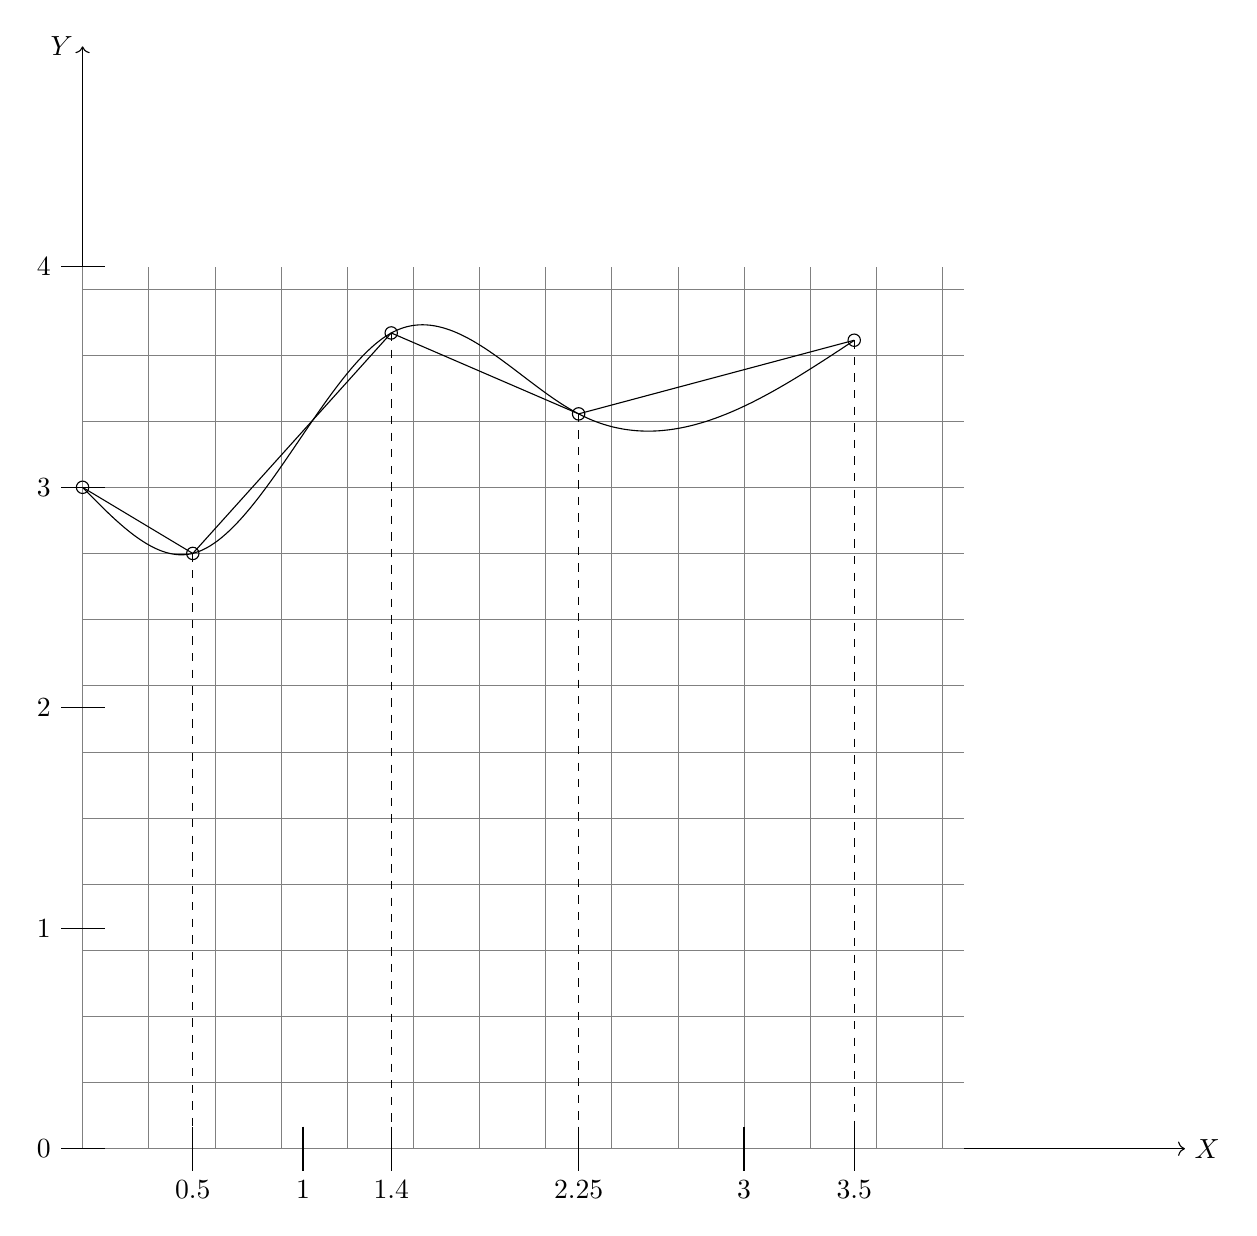
\begin{tikzpicture}
\begin{scope}[scale=2.8]

\draw[thin, ->] (0,0) -- (5,0) node[right] {$X$};
\draw[thin, ->] (0,0) -- (0,5) node[left] {$Y$};
\draw[very thin,color=gray] (0,0) grid[xstep=0.3,ystep=0.3] (4,4);
\foreach \x\xtext in {0.5,1,1.4,2.25,3,3.5} 
\draw (\x,0.1) -- (\x,-0.1) node[below] {$\xtext$};
\foreach \y\ytext in {0,2,1,3,4} 
\draw (0.1,\y) -- (-0.1,\y) node[left] {$\ytext$};
\draw[domain=0:0.5, smooth] plot ({\x},{(1.6949*(\x)*(\x)*(\x))+0+(-1.0237*(\x))+3});
\draw[domain=0.5:1.4, smooth] plot ({\x},{(-1.7586*(\x)*(\x)*(\x))+(5.1803*(\x)*(\x))+(-3.6139*(\x))+3.4317});
\draw[domain=1.4:2.25, smooth] plot ({\x},{(1.2359*(\x)*(\x)*(\x))-(7.3967*(\x)*(\x))+(13.9939*(\x))-4.7853});
\draw[domain=2.25:3.5, smooth] plot ({\x},{(-0.2522*(\x)*(\x)*(\x))+(2.6479*(\x)*(\x))-(8.6065*(\x))+12.1651});
\draw (0,3) circle (0.8pt);
\draw (0.5,2.7) circle (0.8pt);
\draw (1.4,3.7) circle (0.8pt);
\draw (2.25,3.333) circle (0.8pt);
\draw (3.5,3.667) circle (0.8pt);
\draw[thin,dashed] (0.5,2.7) -- (0.5,0);
\draw[thin,dashed] (1.4,3.7)  -- (1.4,0) ;
\draw[thin,dashed]  (2.25,3.333) --  (2.25,0);
\draw[thin,dashed] (3.5,3.667) -- (3.5,0);

\draw[thin]  (0,3) --  (0.5,2.7);
\draw[thin]  (0.5,2.7) --  (1.4,3.7);
\draw[thin]  (1.4,3.7) --  (2.25,3.333);
\draw[thin]  (2.25,3.333) --  (3.5,3.667);

\end{scope};
\end{tikzpicture}

\newpage
\subsection{Анализ и расчёт погрешности кубического сплайна}
Проводя оценки для функций разных классов. Если S(x)
эрмитов кубический сплайн интерполирует на сетке функцию f(x) то имеют место оценки:
\begin{center}
$|S(x)-f(x)| \leq R$
\end{center}
Поскольку функция является достаточно гладкой , то её можно упростить до
\begin{center}
$|S(x)-f(x)| \leq \frac{1}{384} h^4|f''''(x)|$
\end{center}
Из представленной формулы видно, что нам неизвеста функция f(x), с которой изначально были взяты координаты. Следственно для оценки погрешности нам необходимо рассчитать только правую часть неравенства. В этой части тоже присутствует неизвестная нам функция. От которой необходимо взять четвёртую производную.
\begin{center}
$N(x)=A_0+A_1(x-x_0)+A_2(x-x_0)(x-x_1)+A_3(x-x_0)(x-x_1)(x-x_2)+A_4(x-x_0)(x-x_1)(x-x_2)(x-x_3)$
\end{center}

\begin{center}
$f(x_i; x_{i+1}; ... ; x_{j+k-1}; x_{j+k-1} = \frac{f(x_i; x_{i+1}; ... ; x_{j+k-1}; x_{j+k-1}-f(x_i; x_{i+1}; ... ; x_{j+k-1})}{x_{j+k}-x_j}$
\end{center}

\end{center}
Переменная h есть разница ближайшей табличной координаты и координаты просчитываемой точки погрешности.
\begin{center}
$h=|x_v-x_b|$
\parskip=3mm

$F'1=\frac{Y2-Y1}{X2-X1}$ ; $F'2=\frac{Y3-Y2}{X3-X2}$ ;  $F'3=\frac{Y4-Y3}{X4-X3}$ ;$F'41=\frac{Y5-Y4}{X5-X4}$ ;\\
$F'1=-0.6$ ; $F'2=1.1111$ ; $F'3=-0.4318$;$F'4=0.2672;\\
$F''1=\frac{F'2-F'1}{X3-X1}$  ;  $F''2=\frac{F'3-F'2}{X4-X2}$  ;  $F''3=\frac{F'4-F'3}{X5-X3}$ ;\\
$F''1=1.2222$ ; $F''2=-0.86$ ; $F''3=0.3328$;\\
$F'''1=\frac{F''2-F''1}{X4-X1}$ ; $F'''2=\frac{F''3-F''1}{X5-X2}$ ;\\
$F'''1=-0.9351$ ; $F'''2=0.4048$;\\
$F''''1=\frac{F'''2-F'''1}{X5-X1}$ ;\\
$F''''1=0.3828$;\\
\end{center}\\



\newpage      
\subsection{Интерполяция встроенными методами.}
\begin{flushleft}
В математическом пакете «SciLab» можно провести интерполяцию пользуясь парой команд:\\
d = splin(x,y,”method”);\\
is = interp(xx,x,y,d);\\
Где $x=[x_1,x_1,...,x_n_-_1,x_1]$\\
y – значения функции в узлах интерполяции\\
is – значения интерполянта (кубического сплайна,\\ интерполирующего заданную функцию) вычисленные в точках xx .\\
”method” – параметр, отвечающий за граничное условие, налагаеме на интерполянт\\
Граничные условия, соответствющие различным параметрам:\\
1)”natural”-производные в точках x1,xn интерполянты равны нулю\\
2)”clamped”-явное задание производных в точках $x_1,x_n$\\
3)”not\_a\_knot”-третья производная слева и справа равна для точек $x_2$,$x_n_-_1$\\
4) ”fast” – «быстрый» расчет сплайна на основе обычной интерполяции кубическим полиномом\\
5) ”monotone” – на интервалах между узлами интерполяции интерполянт является монотонным\\
Для построения графиков интерполянтов, полученных различными методами будем применять код общего вида, подставляя нужный параметр:\\
xx=[0:0.01:3.5];\\
x=[0,0.5,1.4,2.25,3.5];\\
y=[3.0,2.7,3.7,3.333,3.667];\\
d=splin(x,y,”parameter”);\\
is=interp(xx,x,y,d);\\
plot(xx,is);\\
plot(x,y,”red o”);\\
\end{flushleft}



\begin{figure}[H]
\begin{minipage}[h]{0.47\linewidth}
\center{\includegraphics[width=1\linewidth]{10.PNG}} a) \\
\end{minipage}
\hfill
\begin{minipage}[h]{0.47\linewidth}
\center{\includegraphics[width=1\linewidth]{11.PNG}} \\b)
\end{minipage}
\vfill
\begin{minipage}[h]{0.47\linewidth}
\center{\includegraphics[width=1\linewidth]{12.PNG}} c) \\
\end{minipage}
\hfill
\begin{minipage}[h]{0.47\linewidth}
\center{\includegraphics[width=1\linewidth]{13.PNG}} d) \\
\end{minipage}
\caption{ a) Интерполянт, полученный с помощью ”natural”\\ b)
Интерполянт, полученный с помощью ”fast”\\ c) Интерполянт, полученный с помощью ”monotone” \\d) Интерполянт, полученный с помощью ”clamped” (2,3)}
\label{ris:experimentalcorrelationsignals}
\end{figure}

\newpage
\begin{flushleft}
\section{Задача оптимального распределения неоднородных ресурсов.}
Требуется решить следующую задачу оптимального распределения неоднородных ресурсов. Пусть в распоряжении завода железобетонных изделий\\ (ЖБИ) имеется m видов сырья (песок, щебень, цемент) в объемах ${\bf a_i}$  .Требуется произвести продукцию {\bf n} видов. Дана технологическая норма $c_ij$  требления отдельного i-го вида сырь для изготовления единицы продукции каждого j-го вида. Известна прибыль $\pi_j$  получаема от выпуска единицы продукции j-го вида. Требуется определить, какую продукцию и в каком количестве должен производить завод ЖБИ, чтобы получить максимальную прибыль.\\
{\bfИсходные данные:}\\
\end{flushleft}
\begin{figure}[h]
\center{\includegraphics[width=1\linewidth]{2.PNG}}  \\
\end{figure}

\newpage
\begin{flushleft}
Листинг:\\
C=[4,4,4,6;4,6,6,3;6,4,5,8];\\
b=[14;12;35];\\
ci=[0;0;0;0];\\
cs=[];\\
p=[40;55;35;25];\\
[x,lagr,f]=linpro(-p,C,b,ci,cs);\\
\end{flushleft}
\begin{figure}[h]
\center{\includegraphics[width=0.65\linewidth]{15.PNG}}  \\
\end{figure}
Максимальная прибыль в размере 120 д.е. будет получена, если объем производства продукции П1 составит 3 ед.

\newpage
\section{Вывод:}
В ходе работы, были привиты базовые навыки использования математических пакетов, улучшена вёрстка в TEX`e. Иследованна функция, построен сплайн, решена экономическая задача.


\newpage
\begin{thebibliography}{9}
\bibitem{book1} Scilab: Решение инженерных и математических задач / Е. Р. Алексеев,
О. В. Чеснокова, Е. А. Рудченко. — М. : ALT Linux ; БИНОМ. Лаборатория
знаний, 2008. — 260 с. : ил. ; 8 с. цв. вклейки.— (Библиотека ALT Linux).
\bibitem{book2} Андриевский А.Б., Андриевский Б.Р., Капитонов А.А.,
Фрадков А.Л. Решение инженерных задач в среде Scilab. Учебное
пособие.— СПб.: НИУ ИТМО, 2013. — 97 с.
\bibitem{book3}Решение задач оптимизации средствами Scilab и Excel : Методические
указания к лабораторной работе по дисциплине «Математическая
экономика» / Уфимск. гос. авиац. техн. ун-т; Сост.: Л.М. Бакусов,
О.В. Кондратьева - Уфа, 2011. - 33 с.
\bibitem{book4} https://ru.wikipedia.org/wiki/Интерполяционный\_многочлен\_Лагранжа
\bibitem{book5}Калиткин. Численные методы. М.,Мир, 1980.
\bibitem{book6}Ю.С. Завьялов. Методы сплайн-функций. М.Наука, 1980.
\end{thebibliography}
\end{document}

